% Options for packages loaded elsewhere
\PassOptionsToPackage{unicode}{hyperref}
\PassOptionsToPackage{hyphens}{url}
%
\documentclass[
]{book}
\usepackage{amsmath,amssymb}
\usepackage{iftex}
\ifPDFTeX
  \usepackage[T1]{fontenc}
  \usepackage[utf8]{inputenc}
  \usepackage{textcomp} % provide euro and other symbols
\else % if luatex or xetex
  \usepackage{unicode-math} % this also loads fontspec
  \defaultfontfeatures{Scale=MatchLowercase}
  \defaultfontfeatures[\rmfamily]{Ligatures=TeX,Scale=1}
\fi
\usepackage{lmodern}
\ifPDFTeX\else
  % xetex/luatex font selection
\fi
% Use upquote if available, for straight quotes in verbatim environments
\IfFileExists{upquote.sty}{\usepackage{upquote}}{}
\IfFileExists{microtype.sty}{% use microtype if available
  \usepackage[]{microtype}
  \UseMicrotypeSet[protrusion]{basicmath} % disable protrusion for tt fonts
}{}
\makeatletter
\@ifundefined{KOMAClassName}{% if non-KOMA class
  \IfFileExists{parskip.sty}{%
    \usepackage{parskip}
  }{% else
    \setlength{\parindent}{0pt}
    \setlength{\parskip}{6pt plus 2pt minus 1pt}}
}{% if KOMA class
  \KOMAoptions{parskip=half}}
\makeatother
\usepackage{xcolor}
\usepackage{color}
\usepackage{fancyvrb}
\newcommand{\VerbBar}{|}
\newcommand{\VERB}{\Verb[commandchars=\\\{\}]}
\DefineVerbatimEnvironment{Highlighting}{Verbatim}{commandchars=\\\{\}}
% Add ',fontsize=\small' for more characters per line
\usepackage{framed}
\definecolor{shadecolor}{RGB}{248,248,248}
\newenvironment{Shaded}{\begin{snugshade}}{\end{snugshade}}
\newcommand{\AlertTok}[1]{\textcolor[rgb]{0.94,0.16,0.16}{#1}}
\newcommand{\AnnotationTok}[1]{\textcolor[rgb]{0.56,0.35,0.01}{\textbf{\textit{#1}}}}
\newcommand{\AttributeTok}[1]{\textcolor[rgb]{0.13,0.29,0.53}{#1}}
\newcommand{\BaseNTok}[1]{\textcolor[rgb]{0.00,0.00,0.81}{#1}}
\newcommand{\BuiltInTok}[1]{#1}
\newcommand{\CharTok}[1]{\textcolor[rgb]{0.31,0.60,0.02}{#1}}
\newcommand{\CommentTok}[1]{\textcolor[rgb]{0.56,0.35,0.01}{\textit{#1}}}
\newcommand{\CommentVarTok}[1]{\textcolor[rgb]{0.56,0.35,0.01}{\textbf{\textit{#1}}}}
\newcommand{\ConstantTok}[1]{\textcolor[rgb]{0.56,0.35,0.01}{#1}}
\newcommand{\ControlFlowTok}[1]{\textcolor[rgb]{0.13,0.29,0.53}{\textbf{#1}}}
\newcommand{\DataTypeTok}[1]{\textcolor[rgb]{0.13,0.29,0.53}{#1}}
\newcommand{\DecValTok}[1]{\textcolor[rgb]{0.00,0.00,0.81}{#1}}
\newcommand{\DocumentationTok}[1]{\textcolor[rgb]{0.56,0.35,0.01}{\textbf{\textit{#1}}}}
\newcommand{\ErrorTok}[1]{\textcolor[rgb]{0.64,0.00,0.00}{\textbf{#1}}}
\newcommand{\ExtensionTok}[1]{#1}
\newcommand{\FloatTok}[1]{\textcolor[rgb]{0.00,0.00,0.81}{#1}}
\newcommand{\FunctionTok}[1]{\textcolor[rgb]{0.13,0.29,0.53}{\textbf{#1}}}
\newcommand{\ImportTok}[1]{#1}
\newcommand{\InformationTok}[1]{\textcolor[rgb]{0.56,0.35,0.01}{\textbf{\textit{#1}}}}
\newcommand{\KeywordTok}[1]{\textcolor[rgb]{0.13,0.29,0.53}{\textbf{#1}}}
\newcommand{\NormalTok}[1]{#1}
\newcommand{\OperatorTok}[1]{\textcolor[rgb]{0.81,0.36,0.00}{\textbf{#1}}}
\newcommand{\OtherTok}[1]{\textcolor[rgb]{0.56,0.35,0.01}{#1}}
\newcommand{\PreprocessorTok}[1]{\textcolor[rgb]{0.56,0.35,0.01}{\textit{#1}}}
\newcommand{\RegionMarkerTok}[1]{#1}
\newcommand{\SpecialCharTok}[1]{\textcolor[rgb]{0.81,0.36,0.00}{\textbf{#1}}}
\newcommand{\SpecialStringTok}[1]{\textcolor[rgb]{0.31,0.60,0.02}{#1}}
\newcommand{\StringTok}[1]{\textcolor[rgb]{0.31,0.60,0.02}{#1}}
\newcommand{\VariableTok}[1]{\textcolor[rgb]{0.00,0.00,0.00}{#1}}
\newcommand{\VerbatimStringTok}[1]{\textcolor[rgb]{0.31,0.60,0.02}{#1}}
\newcommand{\WarningTok}[1]{\textcolor[rgb]{0.56,0.35,0.01}{\textbf{\textit{#1}}}}
\usepackage{longtable,booktabs,array}
\usepackage{calc} % for calculating minipage widths
% Correct order of tables after \paragraph or \subparagraph
\usepackage{etoolbox}
\makeatletter
\patchcmd\longtable{\par}{\if@noskipsec\mbox{}\fi\par}{}{}
\makeatother
% Allow footnotes in longtable head/foot
\IfFileExists{footnotehyper.sty}{\usepackage{footnotehyper}}{\usepackage{footnote}}
\makesavenoteenv{longtable}
\usepackage{graphicx}
\makeatletter
\def\maxwidth{\ifdim\Gin@nat@width>\linewidth\linewidth\else\Gin@nat@width\fi}
\def\maxheight{\ifdim\Gin@nat@height>\textheight\textheight\else\Gin@nat@height\fi}
\makeatother
% Scale images if necessary, so that they will not overflow the page
% margins by default, and it is still possible to overwrite the defaults
% using explicit options in \includegraphics[width, height, ...]{}
\setkeys{Gin}{width=\maxwidth,height=\maxheight,keepaspectratio}
% Set default figure placement to htbp
\makeatletter
\def\fps@figure{htbp}
\makeatother
\setlength{\emergencystretch}{3em} % prevent overfull lines
\providecommand{\tightlist}{%
  \setlength{\itemsep}{0pt}\setlength{\parskip}{0pt}}
\setcounter{secnumdepth}{5}
\usepackage{booktabs}
\usepackage{amsthm}
\makeatletter
\def\thm@space@setup{%
  \thm@preskip=8pt plus 2pt minus 4pt
  \thm@postskip=\thm@preskip
}
\makeatother
\ifLuaTeX
  \usepackage{selnolig}  % disable illegal ligatures
\fi
\usepackage[]{natbib}
\bibliographystyle{apalike}
\usepackage{bookmark}
\IfFileExists{xurl.sty}{\usepackage{xurl}}{} % add URL line breaks if available
\urlstyle{same}
\hypersetup{
  pdftitle={Understanding Uncertainty Course Notes},
  pdfauthor={Jeffrey Woo},
  hidelinks,
  pdfcreator={LaTeX via pandoc}}

\title{Understanding Uncertainty Course Notes}
\author{Jeffrey Woo}
\date{2025-06-09}

\begin{document}
\maketitle

{
\setcounter{tocdepth}{1}
\tableofcontents
}
\chapter*{Preface}\label{preface}
\addcontentsline{toc}{chapter}{Preface}

The examples in this preface is based on OpenIntro Statistics (Diez, Ceytinka-Rundel, Barr), Chapter 9.4 and 9.5, which provide more background information. You can access the book for free at \url{https://www.openintro.org/book/os/}

The main goal using data science is to understand data. Broadly speaking, this will involve building a statistical model for predicting, or estimating a response variable based on one or more predictors. Such models are used in a wide variety of fields such as finance, medicine, public policy, sports, and so on. We will look a couple of examples.

\section{Examples}\label{examples}

\subsection{Example 1: Mario Kart Auction Prices}\label{example-1-mario-kart-auction-prices}

In this first example, we will look at Ebay auctions of a video game called Mario Kart that is played on Nintendo Wii. We want to predict the price of an auction based on whether the game is new or not, whether the auction's main photo is a stock photo, the duration of the auction in days, and the number of Wii wheels included with the auction.

A model that we can use for this example is the linear regression model:

\begin{Shaded}
\begin{Highlighting}[]
\FunctionTok{library}\NormalTok{(openintro)}

\NormalTok{Data}\OtherTok{\textless{}{-}}\NormalTok{mariokart}
\DocumentationTok{\#\#fit model}
\NormalTok{result}\OtherTok{\textless{}{-}}\FunctionTok{lm}\NormalTok{(total\_pr}\SpecialCharTok{\textasciitilde{}}\NormalTok{cond}\SpecialCharTok{+}\NormalTok{stock\_photo}\SpecialCharTok{+}\NormalTok{duration}\SpecialCharTok{+}\NormalTok{wheels, }\AttributeTok{data=}\NormalTok{Data)}
\end{Highlighting}
\end{Shaded}

Generally speaking, a linear regression equation takes the following form:

\[
\hat{y} = \hat{\beta}_0 + \hat{\beta}_1 x_1 + \hat{\beta}_2 x_2 + \cdots + \hat{\beta}_k x_k
\]

where \(\hat{y}\) denotes the predicted value of the response variable, the price of the action in this example, \(x_1, x_2, \cdots, x_k\) denote the values of the predictors. This is example, we have: \(x_1\) for whether the game is new or not, \(x_2\) for whether the auction's main photo is a stock photo, \(x_3\) for the duration of the auction in days, and \(x_4\) for the number of Wii wheels included with the auction. \(\hat{\beta}_0, \hat{\beta}_1, \cdots, \hat{\beta}_k\) represent the estimated regression parameters. If we know what these values are, we can easily plug in the values of the predictors to obtain the predicted price of the auction.

Fitting the model in R, we obtain the estimated regression parameters:

\begin{Shaded}
\begin{Highlighting}[]
\DocumentationTok{\#\#get estimated regression parameters}
\NormalTok{result}
\end{Highlighting}
\end{Shaded}

\begin{verbatim}
## 
## Call:
## lm(formula = total_pr ~ cond + stock_photo + duration + wheels, 
##     data = Data)
## 
## Coefficients:
##    (Intercept)        condused  stock_photoyes        duration          wheels  
##        43.5201         -2.5816         -6.7542          0.3788          9.9476
\end{verbatim}

so we have:

\[
\hat{y} = 43.5201 - 2.5816 x_1 - 6.7542 x_2 + 0.3788 x_3 + 9.9476 x_4
\]

So for an auction for Mario Kart game that is used, that uses a stock photo, is listed for 2 days, and comes with 0 wheels, the predicted price will be \(\hat{y} = 43.5201 - 2.5816 - 6.7542 + 0.3788 \times 2 = 34.94\) or about 35 dollars.

\subsection{Example 2: Job Application Callback Rates}\label{example-2-job-application-callback-rates}

In this example, we look at data from an experiment that sought to evaluate the effect of race and gender on job application callback rates. For the experiment, researchers created fake resumes to job postings in Boston and Chicago to see which resumes resulted in a callback. The fake resumes included relevant information such as the applicant's educational attainment, how many year's of experience the applicant as well as a first and last name. The names on the fake resume were meant to imply the applicant's race and gender. Only two races were considered (Black or White) and only two genders were considered (Make or Female) for the experiment.

Prior to the experiment, the researchers conducted surveys to check for racial and gender associations for the names on the fake resumes; only names that passed a certain threshold from the surveys were included in the experiment.

A model that can be used in this example is the logistic regression model

\begin{Shaded}
\begin{Highlighting}[]
\NormalTok{Data2}\OtherTok{\textless{}{-}}\NormalTok{resume}
\DocumentationTok{\#\#fit model}
\NormalTok{result2}\OtherTok{\textless{}{-}}\FunctionTok{glm}\NormalTok{(received\_callback}\SpecialCharTok{\textasciitilde{}}\NormalTok{job\_city }\SpecialCharTok{+}\NormalTok{ college\_degree}\SpecialCharTok{+}\NormalTok{years\_experience}\SpecialCharTok{+}\NormalTok{race}\SpecialCharTok{+}\NormalTok{gender, }\AttributeTok{family=}\StringTok{"binomial"}\NormalTok{, }\AttributeTok{data=}\NormalTok{Data2)}
\end{Highlighting}
\end{Shaded}

Generally speaking, a logistic regression equation takes the following form

\[
\log (\frac{\hat{\pi}}{1-\hat{\pi}}) = \hat{\beta}_0 + \hat{\beta}_1 x_1 + \hat{\beta}_2 x_2 + \cdots + \hat{\beta}_k x_k
\]

where \(\hat{\pi}\) denotes the predicted probability that the applicant receives a call back. \(x_1, x_2, \cdots, x_k\) denote the values of the predictors. This is example, we have: \(x_1\) for which city is the job posting located in, \(x_2\) for whether the applicant has a college degree or not, \(x_3\) for the experience of the applicant, \(x_4\) for associated race of the applicant, and \(x_5\) for the associated gender of the applicant. Similar to linear regression, \(\hat{\beta}_0, \hat{\beta}_1, \cdots, \hat{\beta}_k\) represent the estimated regression parameters. If we know what these values are, we can easily plug in the values of the predictors to obtain the predicted probability for an applicant with those characteristics to receive a callback.

Fitting the model in R, we obtain the estimated regression parameters

\begin{Shaded}
\begin{Highlighting}[]
\DocumentationTok{\#\#get estimated regression parameters}
\NormalTok{result2}
\end{Highlighting}
\end{Shaded}

\begin{verbatim}
## 
## Call:  glm(formula = received_callback ~ job_city + college_degree + 
##     years_experience + race + gender, family = "binomial", data = Data2)
## 
## Coefficients:
##      (Intercept)   job_cityChicago    college_degree  years_experience  
##         -2.63974          -0.39206          -0.06550           0.03152  
##        racewhite           genderm  
##          0.44299          -0.22814  
## 
## Degrees of Freedom: 4869 Total (i.e. Null);  4864 Residual
## Null Deviance:       2727 
## Residual Deviance: 2680  AIC: 2692
\end{verbatim}

so we have

\[
\log (\frac{\hat{\pi}}{1-\hat{\pi}}) = -2.63974 - 0.39206 x_1 - 0.0655 x_2 + 0.03152 x_3 + 0.44299 x_4 - 0.22814 x_5
\]

So for an applicant in Boston, who has a college degree, has 10 years of experience and has a name that is associated with being a Black male, the logistic regression equation becomes \(\log (\frac{\hat{\pi}}{1-\hat{\pi}}) = -2.63974 - 0.0655 + 0.03152 \times 10 - 0.22814 = -2.61818\). Doing a little bit of algebra to solve, we get \(\hat{\pi} = 0.06797751\). Such an applicant has about a 6.8 percent chance of receiving a callback.

\section{How were Estimated Parameters Calculated?}\label{how-were-estimated-parameters-calculated}

In the two examples, notice how I used some R functions, supplied the names of the variables, and the R functions generated the values of the estimated parameters? One thing you will learn is how the functions actually calculate these numbers. It turns out that these calculations are based on foundational concepts associated with measures of uncertainty, probability, and expected values. We will be learning about these concepts in this class.

Why do we want to know how these calculations are performed? So that we understand the intuition and logic behind how these models are built. It becomes a lot easier to work with these models when we understand their logic (for example, we know when these models can be used or cannot be used, we know what steps to take when we notice our data have certain characteristics, etc), instead of memorizing a bunch of steps.

When presenting models and data to people, some people may occasionally questions our methods and models. Why should we trust the model? Should we trust these numbers that seem to come out from some black box?

Notice we used two different models, linear regression and logistic regression, for examples 1 and 2. Why did we use these models? Could we have swapped the type of model used in these examples? The answer is actually no. One of the main considerations when deciding what model to use is to identify if our response variable is quantitative or categorical. You will learn why the linear regression model works when the response variable is quantitative, and why the logistic regression model works when the response variable is categorical.

\section{The Course: Understanding Uncertainty}\label{the-course-understanding-uncertainty}

As mentioned in the previous section, we will be learning about foundational concepts associated with measures of uncertainty, probability, and expected values. All of these concepts will then help explain the intuition and how statistical models are built.

At the end of the course, we will apply these concepts and revisit the linear regression and logistic regression models. These are two of the most widely used models used in data science, as they are relatively easier to understand and explain. More modern methods (that you will learn about in future classes) such as decision trees and neural networks can be viewed as extensions of the linear and logistic regression models.

\chapter{Descriptive Statistics}\label{descriptive-statistics}

\section*{Introduction}\label{introduction}
\addcontentsline{toc}{section}{Introduction}

This module is based on OpenIntro Statistics (Diez, Ceytinka-Rundel, Barr), Chapter 2.1. You can access the book for free at \url{https://www.openintro.org/book/os/} Please note that I cover additional topics, and skip certain topics from the book.

\section{Uncertainty with Data}\label{uncertainty-with-data}

When we are analyzing data, there is always going to be some degree of uncertainty, as there is randomness in a lot of phenomena that we observe in our world. An event is \textbf{random} if individual outcomes of the event are unpredictable. For example, the weight of the next baby born in a local hospital. Without knowing any information about the biological parents, we have a high degree of uncertainty if we try to predict this baby's weight. Even if we know detailed information about the biological parents (for example they are both very tall), we may feel more confident in predicting that the baby is likely to be heavier than average, but we cannot be certain about this prediction.

On the other end hand, an event is \textbf{deterministic} if we can predict individual outcomes of the event with certainty. For example, if we know the length of a cube is 2 inches, we know for sure that its volume is is \(2^3 = 8\) cubic inches, based on rules of mathematics. The volume of a cube with length 2 inches is always going to be 8 cubic inches, so the volume is deterministic.

\emph{Thought question}: think about data that you see in real life. Write these down. Are these data random or deterministic?

We will explore tools to help us quantify uncertainty in data. In this module, we will explore fairly standard tools that are used to describe data and give us an idea about the degree of uncertainty we have in the data. When describing data that is quantitative, we usually describe the following: the shape of its distribution, its average or typical value, and its spread and uncertainty.

\section{Visualizing Data}\label{visualizing-data}

Data visualization is the representation of information in the form of pictures. Imagine have access to weights of all newborn babies at a local hospital. Examining each numerical value could be time consuming. So instead, we can use visualizations to give us an idea about the values of the weights. For example, what weights of newborns are common? What proportion of babies have dangerously low weights (which may indicate health risks)? Good data visualizations can give us such information fairly quickly. Next, we will explore some common visualizations that are used for quantitative (or numerical) variables.

\subsection{Dot Plots}\label{dot-plots}

We will start with a \textbf{dot plot}, as it is the most basic visualization for a quantitative variable. We will use the \texttt{loan50} dataset from the \texttt{openintro} package. The data originally consist of thousands of loans made through the Lending Club platform, but we will randomly select 50 of these loans. Let us study the interest rate the loans the 50 applicants received.

\begin{Shaded}
\begin{Highlighting}[]
\FunctionTok{library}\NormalTok{(tidyverse)}
\FunctionTok{library}\NormalTok{(openintro)}

\DocumentationTok{\#\#create object for data}
\NormalTok{Data}\OtherTok{\textless{}{-}}\NormalTok{loan50}
\end{Highlighting}
\end{Shaded}

For simplicity, we will round the numerical values of the interest rates to the nearest whole number:

\begin{Shaded}
\begin{Highlighting}[]
\DocumentationTok{\#\#round interest rate to whole number}
\NormalTok{Data}\OtherTok{\textless{}{-}}\NormalTok{ Data}\SpecialCharTok{\%\textgreater{}\%}
  \FunctionTok{mutate}\NormalTok{(}\AttributeTok{r\_int\_rate =} \FunctionTok{round}\NormalTok{(interest\_rate))}
\end{Highlighting}
\end{Shaded}

We can create the corresponding dot plot, per Figure \ref{fig:dotplot}:

\begin{Shaded}
\begin{Highlighting}[]
\DocumentationTok{\#\#dotplot}
\FunctionTok{ggplot}\NormalTok{(Data,}\FunctionTok{aes}\NormalTok{(}\AttributeTok{x=}\NormalTok{r\_int\_rate))}\SpecialCharTok{+}
  \FunctionTok{geom\_dotplot}\NormalTok{(}\AttributeTok{binwidth=}\DecValTok{1}\NormalTok{)}\SpecialCharTok{+}
  \FunctionTok{theme}\NormalTok{(}
    \AttributeTok{axis.text.y =} \FunctionTok{element\_blank}\NormalTok{(),  }\CommentTok{\# Remove y{-}axis labels}
    \AttributeTok{axis.title.y =} \FunctionTok{element\_blank}\NormalTok{(), }\CommentTok{\# Remove y{-}axis title}
    \AttributeTok{axis.ticks.y =} \FunctionTok{element\_blank}\NormalTok{()  }\CommentTok{\# Remove y{-}axis ticks}
\NormalTok{  )}\SpecialCharTok{+} 
  \FunctionTok{labs}\NormalTok{(}\AttributeTok{x=}\StringTok{"Interest Rates (Rounded)"}\NormalTok{)}
\end{Highlighting}
\end{Shaded}

\begin{figure}
\centering
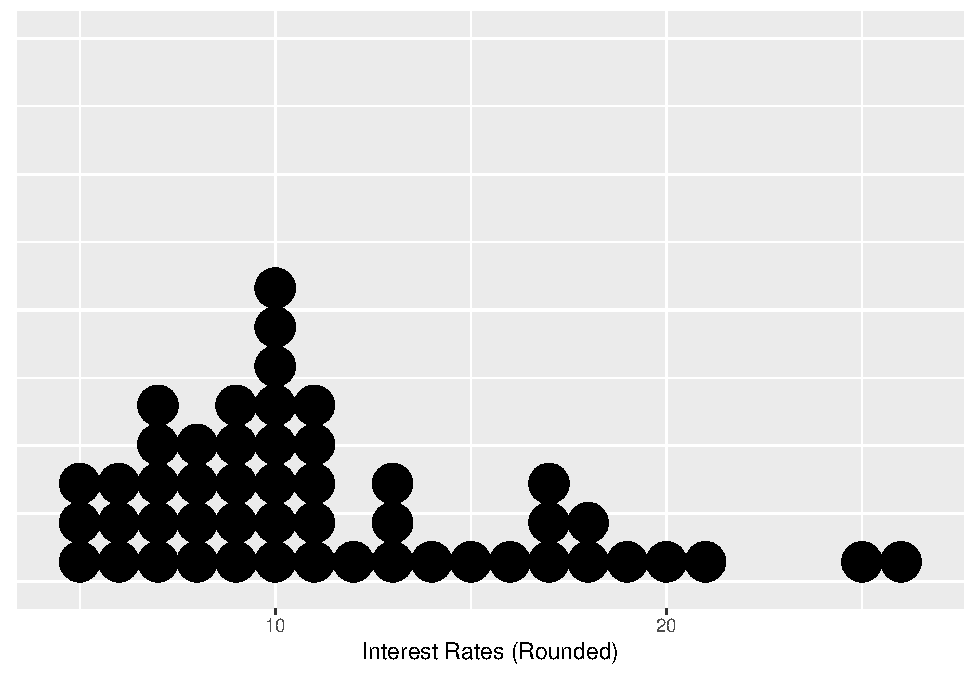
\includegraphics{bookdown-demo_files/figure-latex/dotplot-1.pdf}
\caption{\label{fig:dotplot}Dot Plot for 50 Interest Rates (rounded)}
\end{figure}

Notice there is 1 black dot that corresponds to an interest rate of 20 (presumably in percent), so there is one applicant who has a rounded interest rate of 20 percent. There are 8 black dots that correspond to an interest rate to 10 percent, so there are 8 applicants with a rounded interest rate of 10 percent. So interest rates of 10 percent are much more commonly occurring than interest rate of 20 percent. So we can use the height, or number of dots, to help us glean how often the value of a certain interest rate occurs. Based on this dotplot, interest rates between 5 and 11 percent are common, with higher values being less common.

\emph{Note:} do not get too torn up about the details in the code to produce this dot plot. I have chosen the present the dot plot this way to highlight how we use it, without getting bogged down in the details of how it can be produced. We will not be using dot plots in this class.

\subsection{Histograms}\label{histograms}

It turns out that dot plots are often not useful for large data sets, but they provide the general idea of how other visualizations for larger data sets work. The height of the dots inform us the frequency of those values occurring.

A visualization that is more commonly used for larger data sets is a histogram. Instead of displaying how common each value of the variable exists, we think of the values as belonging to a \textbf{bin} of values. For example, we can create a bin that contains interest rates between 5 and 7.5 percent, another bin containing interest rates between 7.5 and 10 percent, and so on. A few things to note about histograms:

\begin{itemize}
\item
  By convention, values that lie exactly on the boundary of a bin will belong to the lower bin. For example, an interest rate that is exactly 12.5 percent will belong to the bin between 10 and 12.5 percent, and not the bin between 12.5 to 15 percent.
\item
  Each bin should have the same width. In our example, the width is 2.5.
\end{itemize}

We create this histogram (using the original interest rates) below, per Figure \ref{fig:hist}:

\begin{Shaded}
\begin{Highlighting}[]
\DocumentationTok{\#\#set up sequence to specify the bins}
\NormalTok{s25}\OtherTok{\textless{}{-}}\FunctionTok{seq}\NormalTok{(}\DecValTok{5}\NormalTok{,}\FloatTok{27.5}\NormalTok{,}\FloatTok{2.5}\NormalTok{)}

\FunctionTok{ggplot}\NormalTok{(Data,}\FunctionTok{aes}\NormalTok{(}\AttributeTok{x=}\NormalTok{interest\_rate))}\SpecialCharTok{+}
  \FunctionTok{geom\_histogram}\NormalTok{(}\AttributeTok{breaks=}\NormalTok{s25,}\AttributeTok{fill=}\StringTok{"blue"}\NormalTok{,}\AttributeTok{color=}\StringTok{"orange"}\NormalTok{)}\SpecialCharTok{+}
  \FunctionTok{labs}\NormalTok{(}\AttributeTok{x=}\StringTok{"Interest Rate"}\NormalTok{, }\AttributeTok{title=}\StringTok{"Histogram of Interest Rates"}\NormalTok{)}
\end{Highlighting}
\end{Shaded}

\begin{figure}
\centering
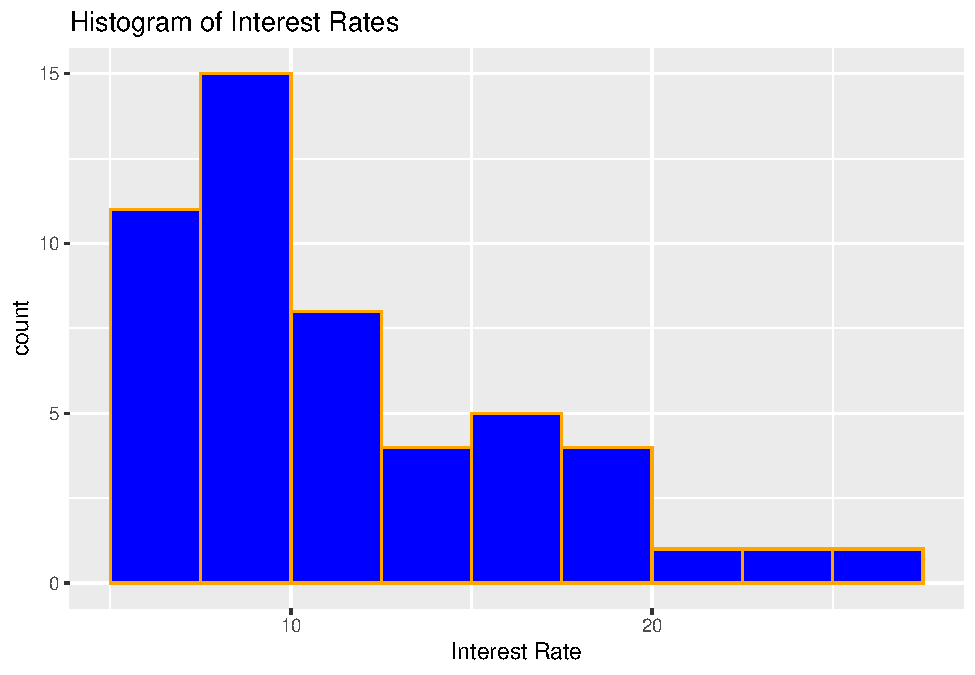
\includegraphics{bookdown-demo_files/figure-latex/hist-1.pdf}
\caption{\label{fig:hist}Historgram for 50 Interest Rates}
\end{figure}

Similar to the dot plot in Figure \ref{fig:dotplot}, the height of the histogram inform us what values are more commonly occurring. We can see from this histogram that interest rates between 5 and 10 percent are common, much more so than loans with interest rates greater than 20 percent. We could say that we have more certainty that a randomly selected loan applicant will have an interest rate between 5 and 10 percent than an interest rate that is greater than 20 percent.

\subsubsection{Shapes of Distribution}\label{shapes-of-distribution}

Histograms can also give us an idea about the \textbf{shape} of the distribution of interest rates. For the histogram in Figure \ref{fig:hist}, most of the loans are less than 15 percent, with only a small number of loans greater than 20 percent. We can say that we have greater certainty that a loan will have an interest rate less than 15 percent. When the data tail off to the right as in our histogram, the shape is said to be \textbf{right-skewed}. When a variable is said to be right-skewed, large values of the variable are much less common than small values of the variable; smaller values are more likely occur.

\begin{itemize}
\item
  If the histogram has the reverse characteristic, i.e.~the data tail off to the left instead, the shape is said to be \textbf{left-skewed}. This implies that small values of the variable are much less common than large values of the variable; larger values are more likely to occur.
\item
  Histograms that trail off similarly in both directions are called \textbf{symmetric}. Large and small values are of the variable are equally likely.
\item
  Histograms that have a peak in the middle, and then trail off on both sides are not only symmetic, but also \textbf{bell-shaped}, or have a \textbf{normal} distribution. Note: it turns out one of the assumptions in linear regression is that the response variable follow a normal distribution. This may seem restrictive, however, we will see in later modules that this assumption is not particular crucial under some circumstances.
\end{itemize}

\emph{Thought question:} Can you think of real life variables that have symmetric, right-skewed, left-skewed distributions? Feel free to search the internet for examples.

\subsubsection{Considerations with Histograms}\label{considerations-with-histograms}

With our interest rate example, you may have noticed that I made a specific choice to the width of the bins when I created the histograms. It turns out that the width of the bins can impact the shape of the histogram, and potentially, how we interpret the histogram.

Consider creating a histogram with bin width of 0.5, instead of 2.5, per Figure \ref{fig:hist05}:

\begin{Shaded}
\begin{Highlighting}[]
\DocumentationTok{\#\#set up sequence to specify the bins. width now 0.5}
\NormalTok{s05}\OtherTok{\textless{}{-}}\FunctionTok{seq}\NormalTok{(}\DecValTok{5}\NormalTok{,}\FloatTok{27.5}\NormalTok{,}\FloatTok{0.5}\NormalTok{)}

\FunctionTok{ggplot}\NormalTok{(Data,}\FunctionTok{aes}\NormalTok{(}\AttributeTok{x=}\NormalTok{interest\_rate))}\SpecialCharTok{+}
  \FunctionTok{geom\_histogram}\NormalTok{(}\AttributeTok{breaks=}\NormalTok{s05,}\AttributeTok{fill=}\StringTok{"blue"}\NormalTok{,}\AttributeTok{color=}\StringTok{"orange"}\NormalTok{)}\SpecialCharTok{+}
  \FunctionTok{labs}\NormalTok{(}\AttributeTok{x=}\StringTok{"Interest Rate"}\NormalTok{, }\AttributeTok{title=}\StringTok{"Histogram of Interest Rates"}\NormalTok{)}
\end{Highlighting}
\end{Shaded}

\begin{figure}
\centering
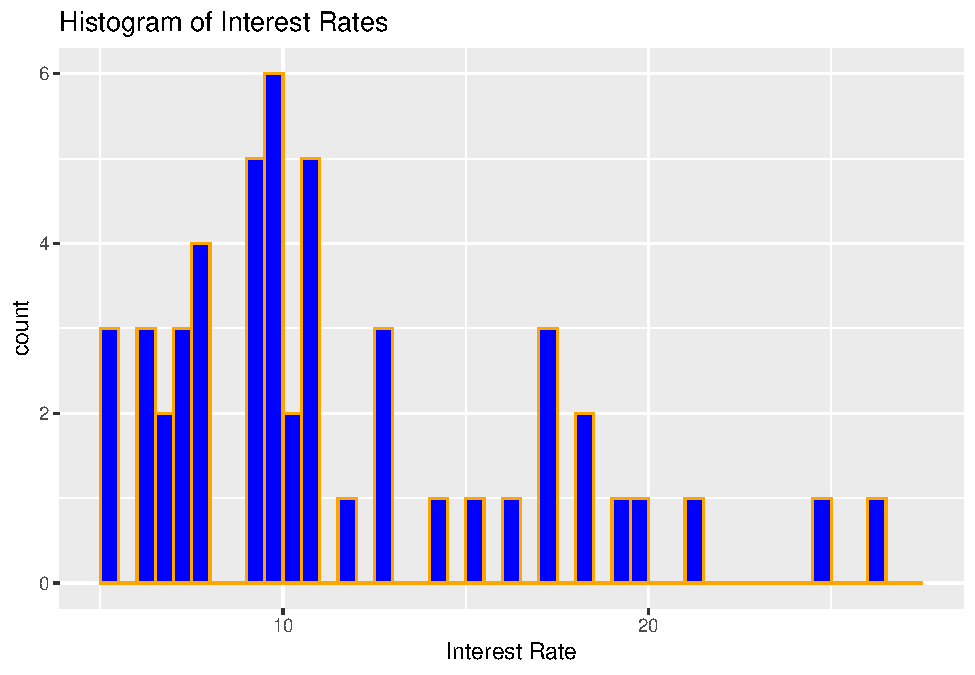
\includegraphics{bookdown-demo_files/figure-latex/hist05-1.pdf}
\caption{\label{fig:hist05}Historgram for 50 Interest Rates, with Bin Width 0.5}
\end{figure}

Comparing Figure \ref{fig:hist05} with Figure \ref{fig:hist}, note the following:

\begin{itemize}
\item
  Visually, the histogram looks more jagged with smaller bin width, whereas the histogram looks smoother with a larger bin width.
\item
  Smaller bin widths may be preferred if we need information about smaller ranges of interest rates. However, it can be difficult to write about general trends.
\item
  Larger bin widths may be more useful if we are trying to look for more general trends in the interest rates.
\end{itemize}

\emph{Thought question}: What happens if we create a histogram with a bin width that is too large?

\subsection{Density Plots}\label{density-plots}

Another visualization for a quantitative variable is a density plot. A density plot can be viewed as a smoothed version of the histogram. We can use the heights to inform us about what values are more common. We create a density plot for the interest rates in Figure \ref{fig:dens}:

\begin{Shaded}
\begin{Highlighting}[]
\DocumentationTok{\#\#density plot}
\FunctionTok{plot}\NormalTok{(}\FunctionTok{density}\NormalTok{(Data}\SpecialCharTok{$}\NormalTok{interest\_rate), }\AttributeTok{main=}\StringTok{"Density Plot of Interest Rates"}\NormalTok{)}
\end{Highlighting}
\end{Shaded}

\begin{figure}
\centering
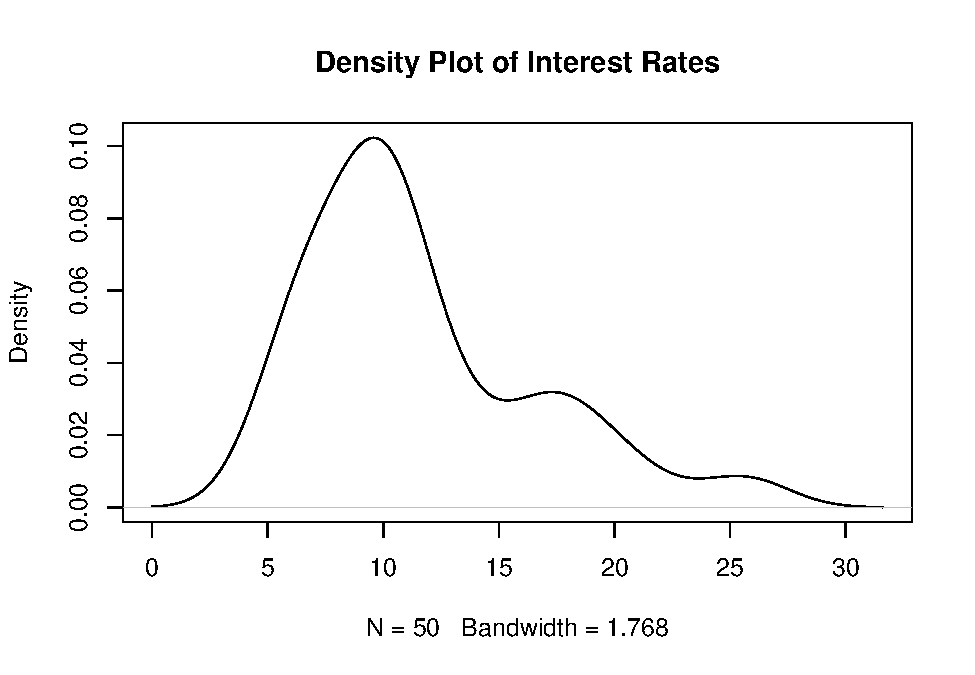
\includegraphics{bookdown-demo_files/figure-latex/dens-1.pdf}
\caption{\label{fig:dens}Density Plot for 50 Interest Rates}
\end{figure}

Based on Figure \ref{fig:dens}, we see that low interest rates (between 5 and 12.5 percent) are much more common and high interest rates (higher than 20 percent). A few things to note about interpreting density plots:

\begin{itemize}
\tightlist
\item
  The area under the density plot is always equals to 1.
\item
  To find the proportion of interest rates that are between two values, for example between 10 and 15 percent, we would integrate this density plot over this range, i.e.~\(\int_{10}^{15} f(x) dx\), where \(f(x)\) is a mathematical equation that describes the density plot.
\item
  The values on the vertical axis do not equal to probabilities (a common misconception).
\end{itemize}

The density plot is found using a method called kernel density estimation (KDE). We will over details about KDE in a later module as we need to cover quite a bit of material before doing so.

\subsubsection{Considerations with Density Plots}\label{considerations-with-density-plots}

Similar to bins and histograms, density plots are affected by the \textbf{bandwidth}. Larger bandwidths lead to smoother density plots, while smaller bandwidths lead to more jagged density plots. We create a density plot that uses a bandwidth that is twice the default in Figure \ref{fig:dens2} below:

\begin{Shaded}
\begin{Highlighting}[]
\FunctionTok{plot}\NormalTok{(}\FunctionTok{density}\NormalTok{(Data}\SpecialCharTok{$}\NormalTok{interest\_rate, }\AttributeTok{adjust=}\DecValTok{2}\NormalTok{), }\AttributeTok{main=}\StringTok{"Density Plot of Interest Rates, with Bandwidth Twice the Default"}\NormalTok{)}
\end{Highlighting}
\end{Shaded}

\begin{figure}
\centering
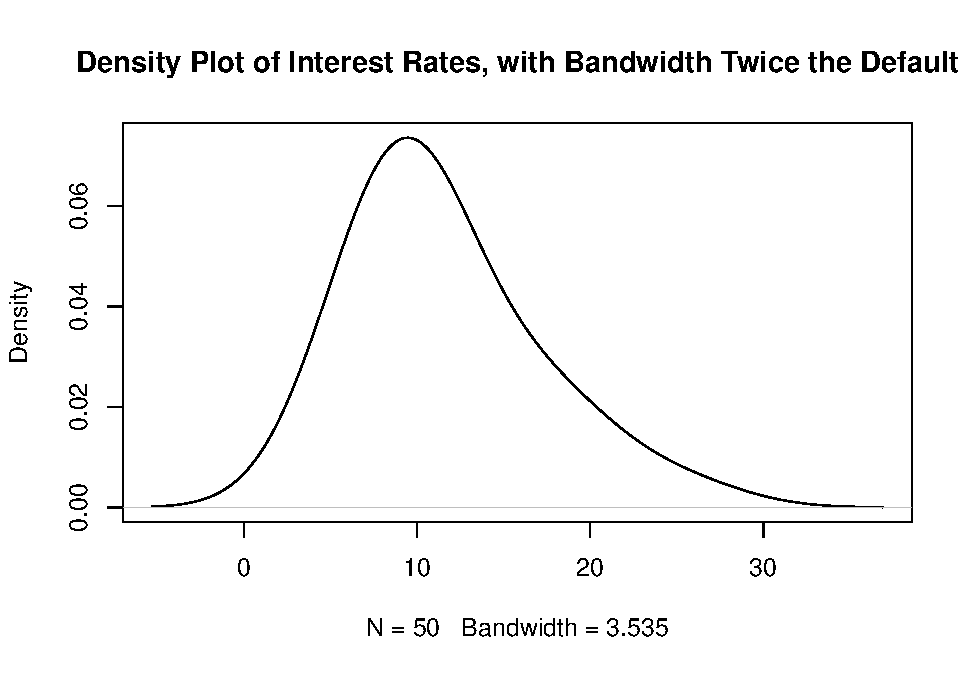
\includegraphics{bookdown-demo_files/figure-latex/dens2-1.pdf}
\caption{\label{fig:dens2}Density Plot for 50 Interest Rates with Larger Bandwidth}
\end{figure}

Notice in Figure \ref{fig:dens2} that the little peak for interest rates between 15 and 20 (which existed in Figures \ref{fig:dens} and also \ref{fig:hist}) no longer exists. Using bandwidths that are too large can smooth out some of these peaks.

\emph{Thought question}: What if we create a density plot with a bandwidth that is too small?

\emph{Thought question}: How are bin widths for histograms and bandwidths for density plots related?

\section{Ordered Statistics}\label{ordered-statistics}

The idea behind ordered statistics is pretty self-explanatory: take your numerical variable, and order the values from smallest to largest. Going back to our example of the interest rates from 50 loan applicants, let \(X\) denote the interest rate. Then \(x_{(1)}\) will denote the interest rate that is the smallest, \(x_{(2)}\) denotes the second smallest interest rate, and \(x_{(50)}\) denotes the largest interest rate in our sample of 50.

\subsection{Quantiles}\label{quantiles}

\textbf{Quantiles} partition the range of numerical data into continuous intervals (groups) with (nearly) equal proportions. Common quartiles have their own names:

\begin{itemize}
\tightlist
\item
  Quartiles: 4 groups
\item
  Percentiles: 100 groups
\end{itemize}

There is one less quantiles than the number of groups. We will go over quartiles in more detail.

\subsubsection{Quartiles}\label{quart}

Quartiles divide the data into 4 groups, and each group has (nearly) equal number of observations. So there will be three quartiles, denoted by \(Q_1, Q_2, Q_3\).

\begin{itemize}
\tightlist
\item
  The first group will have values between negative infinity and \(Q_1\).
\item
  The second group will have values between negative \(Q_1\) and \(Q_2\).
\item
  The third group will have values between negative \(Q_2\) and \(Q_3\).
\item
  The fourth group will have values between negative \(Q_3\) and infinity.
\end{itemize}

\(Q_2\), sometimes called the second quartile, is the easiest value to find. It is also called the \textbf{median} of the data. Going back to our interest rates from the 50 loan applicants. Using our ordered statistics, the median is the middle observation. Since we have an even number of observations, we have two middle observations, \(x_{(25)}\) and \(x_{(26)}\). In this situation, the median will be the average of these two middle observations. Using R, we find the median to be:

\begin{Shaded}
\begin{Highlighting}[]
\FunctionTok{median}\NormalTok{(Data}\SpecialCharTok{$}\NormalTok{interest\_rate)}
\end{Highlighting}
\end{Shaded}

\begin{verbatim}
## [1] 9.93
\end{verbatim}

So half the interest rates are less than 9.93 percent, and half the interest rates are greater than 9.93 percent. You might also recognize another term for the median: the 50th percentile, as 50 percent of the interest rates are less than 9.93.

To find the middle observation(s) based on a sample of size \(n\):

\begin{itemize}
\tightlist
\item
  If \(n\) is even, the 2 middle observations will be position \(\frac{n}{2}\) and \(\frac{n}{2} + 1\) in the ordered statistics.
\item
  If \(n\) is odd, the middle observation will be position \(\frac{n}{2} + 0.5\) in the ordered statistics.
\end{itemize}

\(Q_1\) and \(Q_3\) (also called the first and third quartiles) are found together, after finding \(Q_2\). Note that \(Q_2\) divides the data into two groups. Using our interest rates example, one group contains \(x_{(1)}, \cdots, x_{(25)}\), and another group contains \(x_{(26)}, \cdots, x_{(50)}\). \(Q_1\) is the median of the first group, and \(Q_3\) is the median of the second group. So for our 50 loan applicants:

\begin{itemize}
\tightlist
\item
  \(Q_1\) is \(x_{(13)}\), and
\item
  \(Q_3\) is \(x_{(38)}\).
\end{itemize}

To find these values in R, we could type:

\begin{Shaded}
\begin{Highlighting}[]
\FunctionTok{quantile}\NormalTok{(Data}\SpecialCharTok{$}\NormalTok{interest\_rate, }\AttributeTok{prob=}\FunctionTok{c}\NormalTok{(}\FloatTok{0.25}\NormalTok{,}\FloatTok{0.75}\NormalTok{), }\AttributeTok{type =} \DecValTok{1}\NormalTok{)}
\end{Highlighting}
\end{Shaded}

\begin{verbatim}
##   25%   75% 
##  7.96 14.08
\end{verbatim}

So \(Q_1\) is 7.96 percent, and \(Q_3\) is 14.08 percent. It turns out that \(Q_1\) is also the 25th percentile, and \(Q_3\) is also the 75th percentile, by definition.

Remember we wrote the following earlier:

\begin{itemize}
\tightlist
\item
  The first group will have values between negative infinity and \(Q_1\). So about a quarter of observations are have interest rates less than 7.96 percent.
\item
  The second group will have values between negative \(Q_1\) and \(Q_2\). So about a quarter of observations have interest rates between 7.96 and 9.93 percent.
\item
  The third group will have values between negative \(Q_2\) and \(Q_3\). So about a quarter of observations have interest rates between 9.93 and 14.08 percent.
\item
  The fourth group will have values between negative \(Q_3\) and infinity. So about a quarter of observations have interest rates above 14.08 percent.
\end{itemize}

Note: you may notice that we used \texttt{type\ =\ 1} inside the \texttt{quantile()} function. Using \texttt{type\ =\ 1} gives the values of the first and third quartiles that are based on the method that was just described. There are actually several ways to find quantiles, which may result in slightly differing values, although they all generally meet the definition that \(Q_1\) is the 25th percentile, and \(Q_3\) is the 75th percentile.

\subsubsection{Percentiles}\label{percentiles}

Another common quantile is the percentile. In general the \textbf{k-th percentile} is the value of the data point below which \(k\) percent of observations are found. So in our earlier example, we said that \(Q_3\) of the interest rates is 14.08 percent, and this is also the 75th percentile. So 75 percent of interest rates are less than 14.08 percent.

We will not go over the details of finding percentiles by hand.

\subsection{Box Plots}\label{box-plots}

Another visualization used to summarize quantitative data is the box plot. A \textbf{box plot} summarizes the 5-number summary. The 5 numbers are the minimum, \(Q_1, Q_2, Q_3\), and the maximum. Using our interest rate data, the box plot is shown in Figure \ref{fig:boxplot}:

\begin{Shaded}
\begin{Highlighting}[]
\DocumentationTok{\#\#box plot}
\FunctionTok{ggplot}\NormalTok{(Data,}\FunctionTok{aes}\NormalTok{(}\AttributeTok{y=}\NormalTok{interest\_rate))}\SpecialCharTok{+}
  \FunctionTok{geom\_boxplot}\NormalTok{()}\SpecialCharTok{+}
  \FunctionTok{labs}\NormalTok{(}\AttributeTok{y=}\StringTok{"Interest Rate"}\NormalTok{, }\AttributeTok{title=}\StringTok{"Box Plot of Interest Rates"}\NormalTok{)}
\end{Highlighting}
\end{Shaded}

\begin{figure}
\centering
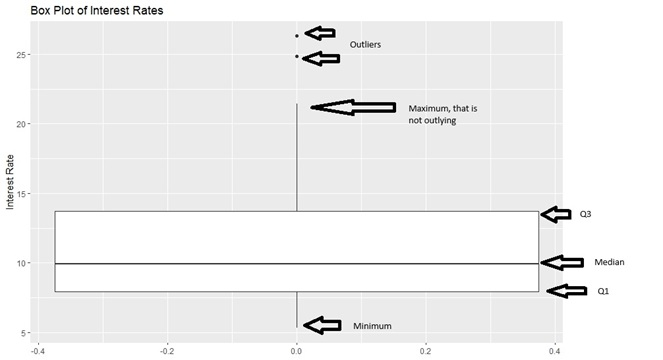
\includegraphics{images/01-boxplot.jpeg}
\caption{\label{fig:boxplot}Box Plot of Interest Rates}
\end{figure}

Some people call a box plot a box and whisker plot.

\begin{itemize}
\tightlist
\item
  The boundaries of the box represent \(Q_1\) and \(Q_3\).
\item
  The thick line in the box represents the median.
\item
  The two whiskers on either side of the box extend to the minimum and maximum, if outliers do not exist. If outliers exist, the whiskers extend to the minimum and maximum values that are not outliers.
\end{itemize}

Generally, when we have one quantitative variable, an outlier is an observation whose numerical value is far away from the rest of the data. In other words, it is a lot smaller or larger relative to the rest of the data.

So for our 50 loans, there are two loan applicants with interest rates around 25 percent that are flagged as being a lot larger than the rest of the loans, which is reasonable since most of the loans are a lot smaller than 20 percent.

We will not go over the details of how outliers are determined in box plots. If you are interested, you can read Chapter 2.1.5 from OpenIntro Statistics (Diez, Ceytinka-Rundel, Barr).

Notice how much further large values (\(Q_3\) and maximum) are from the median, compared to the distance of the small values (\(Q_1\) and minimum) from the median. This indicates that the distribution of interest rates are right-skewed. Compare the boxplot of the interest rates in Figure \ref{fig:boxplot} with its corresponding histogram (Figure \ref{fig:hist}) and density plot (Figure \ref{fig:dens}).

\emph{Thought question}: can you sketch a box plot that represents a variable that is left-skewed? How about a variable that is symmetric?

\subsection{Empirical Cumulative Distribution Function}\label{empirical-cumulative-distribution-function}

From the previous sections, we can see how we could use histograms, density plots, and box plots to inform us about what proportion of observations take certain values, and the values of the data that correspond to certain percentiles. However, we are limited to quartiles and not any percentile when using box plots, and we need to find areas under the density plot (using integration, not a trivial task), or add up frequencies on a histogram (can be time consuming).

A plot that can easily give us values of the variable that correspond to percentiles is the \textbf{empirical cumulative distribution function (ECDF)} plot.

Let \(X\) denote a random variable, and we have observed \(n\) observations of \(X\) denoted by \(x_1, \cdots, x_n\). Let \(x_{(1)}, \cdots x_{(n)}\) denote the ordered statstics of the \(n\) observations. The ECDF, denoted by \(\hat{F}_n(x)\) is the proportion of sample observations less than or equal to the value \(x\) of the random variable. Mathematically, the ECDF is:

\[
 \hat{F}_n(x) = 
  \begin{cases} 
   0, & \text{for } x < x_{(1)} \\
   \frac{k}{n},       & \text{for } x_{(k)} \leq x < x_{(k+1)}, k = 1, \cdots, n-1\\
   1, & \text{for } x \geq x_{(n)}.
  \end{cases}
\]
We shall use a simple toy example to illustrate how an ECDF is constructed. Suppose we ask 5 people how many times to go to the gym (at least 20 minutes) in a typical work week. The answers are: 3, 0, 1, 5, 3. The random variable \(X\) is how many times a person goes to the gym for at least 20 minutes, and the ordered statistics are \(x_{(1)} = 0, x_{(2)} = 1, x_{(3)} = 3, x_{(4)} = 3, and x_{(5)} = 5\). Using the mathematical definition for the ECDF, we have:

\begin{itemize}
\tightlist
\item
  \(\hat{F}_n(x) = 0\) for \(x < x_{(1)} = 0\).
\item
  \(\hat{F}_n(x) = \frac{1}{5}\) for \(0 \leq x < x_{(2)} = 1\).
\item
  \(\hat{F}_n(x) = \frac{2}{5}\) for \(1 \leq x < x_{(3)} = 3\).
\item
  \(\hat{F}_n(x) = \frac{4}{5}\) for \(3 \leq x < x_{(5)} = 5\). This value is special for this example since we have two observations where \(x=3\).
\item
  \(\hat{F}_n(x) = 1\) for \(x \geq 5\).
\end{itemize}

The corresponding ECDF plot is shown in Figure \ref{fig:ecdf}:

\begin{Shaded}
\begin{Highlighting}[]
\DocumentationTok{\#\#toy data}
\NormalTok{y}\OtherTok{\textless{}{-}}\FunctionTok{c}\NormalTok{(}\DecValTok{3}\NormalTok{, }\DecValTok{0}\NormalTok{, }\DecValTok{1}\NormalTok{, }\DecValTok{5}\NormalTok{, }\DecValTok{3}\NormalTok{)}
\DocumentationTok{\#\#ECDF plot}
\FunctionTok{plot}\NormalTok{(}\FunctionTok{ecdf}\NormalTok{(y), }\AttributeTok{main =} \StringTok{"ECDF for Toy Example"}\NormalTok{)}
\end{Highlighting}
\end{Shaded}

\begin{figure}
\centering
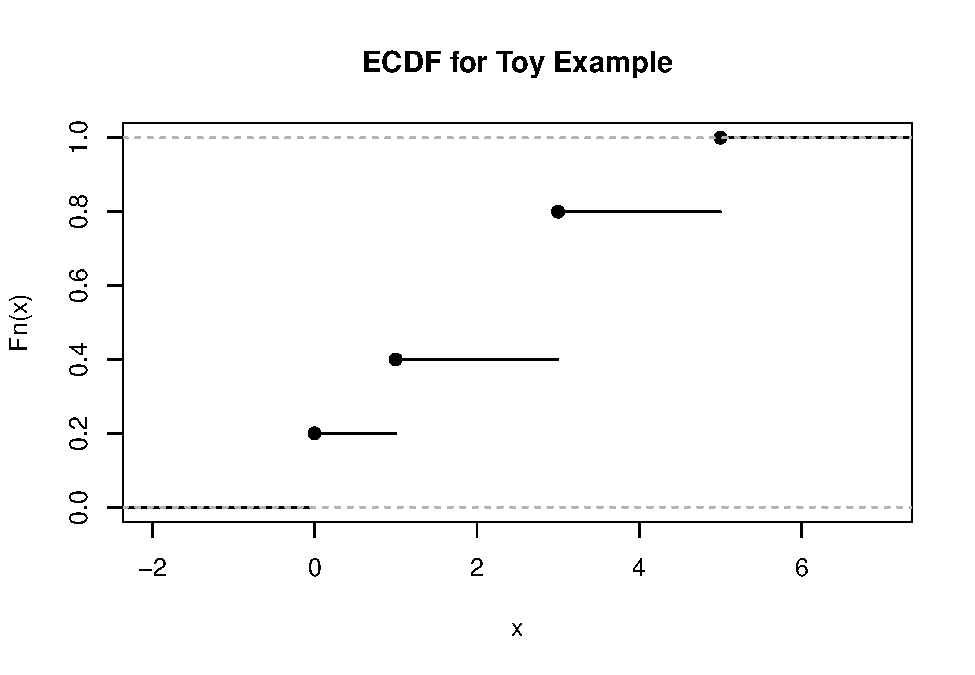
\includegraphics{bookdown-demo_files/figure-latex/ecdf-1.pdf}
\caption{\label{fig:ecdf}ECDF Plot for Toy Example}
\end{figure}

We can easily find percentiles from this plot, for example, the 40th percentile is equal to 1, going to the gym once a week. About 20 percent of observations go to the gym less than 1 time a week.

Next, we create the ECDF plot for the interest rates from the 50 loan applicants.

\begin{Shaded}
\begin{Highlighting}[]
\FunctionTok{plot}\NormalTok{(}\FunctionTok{ecdf}\NormalTok{(Data}\SpecialCharTok{$}\NormalTok{interest\_rate), }\AttributeTok{main =} \StringTok{"ECDF Plot of Interest Rates"}\NormalTok{)}
\FunctionTok{abline}\NormalTok{(}\AttributeTok{h=}\FloatTok{0.8}\NormalTok{)}
\end{Highlighting}
\end{Shaded}

\begin{figure}
\centering
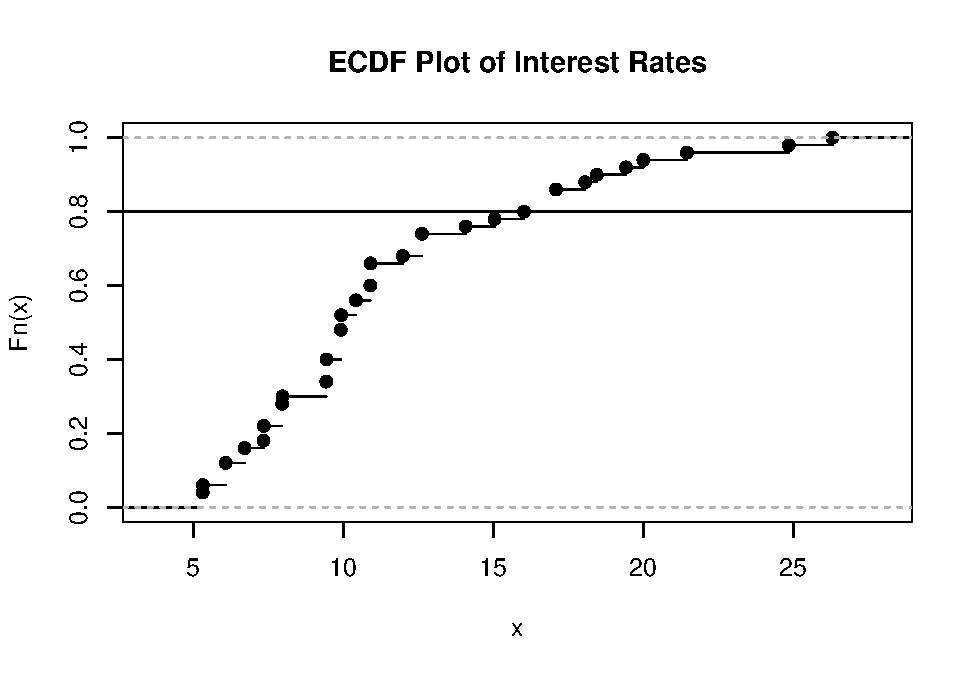
\includegraphics{bookdown-demo_files/figure-latex/ecdfreal-1.pdf}
\caption{\label{fig:ecdfreal}ECDF Plot of Interest Rates}
\end{figure}

I overlaid a horizontal line for the 80th percentile, so we can read on the horizontal axis that this corresponds to an interest rate of about 17 percent. So about 80 percent of loan applicants have an interest rate less than 17 percent.

\emph{Thought question}: try using the histogram and density plot for the interest rates (Figures \ref{fig:hist} and \ref{fig:dens}) to find the interest rate that corresponds to the 80th percentile. Was this easy to perform?

\section{Measures of Centrality}\label{measures-of-centrality}

So far, we have used visualizations to summarize the shape of the distribution of a quantitative variable. Next, we look at common measures of centrality. Loosely speaking, measures of centrality are measures that describe the average or typical value of a quantitative variable. The common measures of centrality are the mean, median, and mode.

\subsection{Mean}\label{mean}

The sample \textbf{mean} is simply the average value of the variable in our sample. The sample mean for a random variable \(X\) is denoted by \(\bar{x}\), and is found by:

\begin{equation} 
\bar{x} = \frac{\sum_{i=1}^n x_i}{n}.
\label{eq:mean}
\end{equation}

So, for our toy example of the 5 people and how often they go to the gym in a week, their sample mean is \(\bar{x} = \frac{3+0+1+5+3}{5} = 2.4\).

\subsection{Median}\label{median}

We went over how to find the median in section \ref{quart}. The \textbf{median} is the value of the middle observation in ordered statistics. It is also called \(Q_2\), the second quartile, and the 50th percentile, so approximately 50 percent of observations have values smaller than the median.

So, for our toy example of the 5 people and how often they go to the gym in a week, their sample median is \(x_{(3)} = 3\). So about 50 percent of people went to gym less than 3 times in a week.

\subsection{Mode}\label{mode}

Another measure is the mode. Mathematically speaking, the \textbf{mode} is the most commonly occurring value in the data. So for our toy example, the mode is 3, since 3 occurs twice and occurs the most often in our data.

\subsection{Considerations}\label{considerations}

A few things to consider when using these measures of centrality:

\begin{itemize}
\item
  The mean is a measure that most people are comfortable with, however, caution needs to be used if the variable is skewed, as extreme outliers and drastically alter the value of the mean. Using our toy example with the gym, suppose the person who visits the gym the most visits 50 times, instead of 5. The numerical value of the sample mean explodes, and does not give a good representation of the central value of how many visits to the gym a person makes in a week. The mean is fine if the variable is symmetric.
\item
  The median is a measure that is recommended for skewed distributions, since the order associated with ordered statistics is not influenced by extreme outliers. Using the gym example, in the previous bullet point, the median is unaffected.
\item
  The mean being larger than the median is an indication that the distribution is right-skewed. Using our interest rate example, we have:
\end{itemize}

\begin{Shaded}
\begin{Highlighting}[]
\FunctionTok{mean}\NormalTok{(Data}\SpecialCharTok{$}\NormalTok{interest\_rate)}
\end{Highlighting}
\end{Shaded}

\begin{verbatim}
## [1] 11.5672
\end{verbatim}

\begin{Shaded}
\begin{Highlighting}[]
\FunctionTok{median}\NormalTok{(Data}\SpecialCharTok{$}\NormalTok{interest\_rate)}
\end{Highlighting}
\end{Shaded}

\begin{verbatim}
## [1] 9.93
\end{verbatim}

which is consistent with the right skew we saw in the histogram and density plot in Figures \ref{fig:hist} and \ref{fig:dens}. Conversely, a left-skewed distribution usually has a mean that is smaller than the median. A symmetric distribution typically has similar values for the mean and median.

\begin{itemize}
\item
  The mean is considered a \textbf{sensitive} measure, since its numerical value can be drastically affected by outliers. The median is considered a \textbf{robust} measure, since its numerical value is more resistant and is less affected by outliers.
\item
  The mathematical definition of mode can be difficult to use for variables that are continuous, since it is likely that there are no observations that have the same value when the variable is continuous. In this instance, the mode typically refers to the bin in the histogram that has is the tallest. So, using the histogram in Figure \ref{fig:hist} for the interest rates, the mode is between 7.5 to 10 percent.
\end{itemize}

\section{Measures of Uncertainty}\label{measures-of-uncertainty}

In the previous sections, we learned about summarizing features a quantitative variable, by using visualizations to summarize its shape, and by using some measures of centrality that describe the average or typical values of the variable. One more feature we can summarize is the spread, associated with the values of a quantitative variable. Measures of spread are considered a way to measure uncertainty. Data that have larger spread have more uncertainty.

\subsection{Variance and Standard Deviation}\label{variance-and-standard-deviation}

One measure of spread is the variance. The sample \textbf{variance} for a random variable \(X\) is denoted by \(s^2\), or sometimes \(s_x^2\), and is found by:

\begin{equation} 
s^2 = \frac{\sum_{i=1}^n (x_i-\bar{x})^2}{n-1}.
\label{eq:variance}
\end{equation}

The variance can be interpreted as the approximate average squared distance of the observations from the mean. The formula in equation \eqref{eq:variance} may look a bit complicated, but let us use the toy example where we asked 5 people how often they go to the gym in a workweek. The answers are: 3, 0, 1, 5, 3, and we had earlier found the sample mean to be \(\bar{x} = 2.4\). To calculate the sample variance:

\[
\begin{split}
s^2 &= \frac{\sum_{i=1}^n (x_i-\bar{x})^2}{n-1}\\
 &= \frac{(3-2.4)^2 + (0-2.4)^2 + (1-2.4)^2 + (5-2.4)^2 + (3-2.4)^2}{5-1} \\
&= 3.8 
\end{split}
\]

Notice what we did in the numerator of equation \eqref{eq:variance}: we take the difference between each observed value from the sample mean, square these differences, then add up the squared differences. We then divide by \(n-1\), rather than \(n\), hence the sample variance being the approximate averaged squared distance of the observations from the mean. There is some nuance in the mathematics as to why we divide by \(n-1\) instead of \(n\), and may not be intuitive as to why we do so. It turns out dividing by \(n-1\) makes the sample variance an unbiased estimator of the true variance in the population (denoted by \(\sigma^2\)) and is more reliable than if we had divided by \(n\). We will go over this in more detail in a later module after covering a few additional concepts.

Larger values of the sample variance indicate that the observations are generally further away from the sample mean, indicating larger spread, and a higher degree of uncertainty about future values.

\emph{Thought question}: What does it mean if the sample variance of a set of observations is 0? Why does this indicate their there is little (or no) uncertainty about the set of observations?

Another related measure is the sample \textbf{standard deviation}, which is the square root of the sample variance. Similar to the variance, larger values indicated more spread in the data.

\subsection{Interquartile Range}\label{interquartile-range}

Another measure of spread is the \textbf{interquartile range (IQR)}, and it is the difference between the third and first queartiles,

\begin{equation} 
IQR = Q_3 - Q_1.
\label{eq:IQR}
\end{equation}

The IQR is considered a robust measure of spread, while the sample variance and standard deviations are considered to be sensitive.

  \bibliography{book.bib,packages.bib}

\end{document}
